\documentclass{beamer}

\usepackage{Haust2017glærur}

\title{Stærðfræðimynstur í tölvunarfræði}
\subtitle{Vika 10, seinni fyrirlestur}

\begin{document}

\begin{frame}
\titlepage
\end{frame}

\section{Inngangur}

\begin{frame}{Í síðasta tíma}
\begin{itemize}
 \item Net
 \item Hagnýting neta
 \item Nokkur hugtök sem tengjast netum
\end{itemize}
\end{frame}

\section{Kosningareiknirit}

\subsection{Regla D'Hondt}

\begin{frame}{Úthlutun fulltrúasæta}
    \begin{itemize}
        \item Ísland er fulltrúalýðræði með flokkakerfi, skipt í kjördæmi
        \item Hvert kjördæmi hefur ákveðinn fjölda kjördæmissæta
        \item Þurfum reiknirit sem getur breytt atkvæðafjölda yfir í þingsætafjölda
        \item Regla D'Hondt er notuð á Íslandi
    \end{itemize}
\end{frame}

\begin{frame}{Atkvæðatölur og þingsæti}
    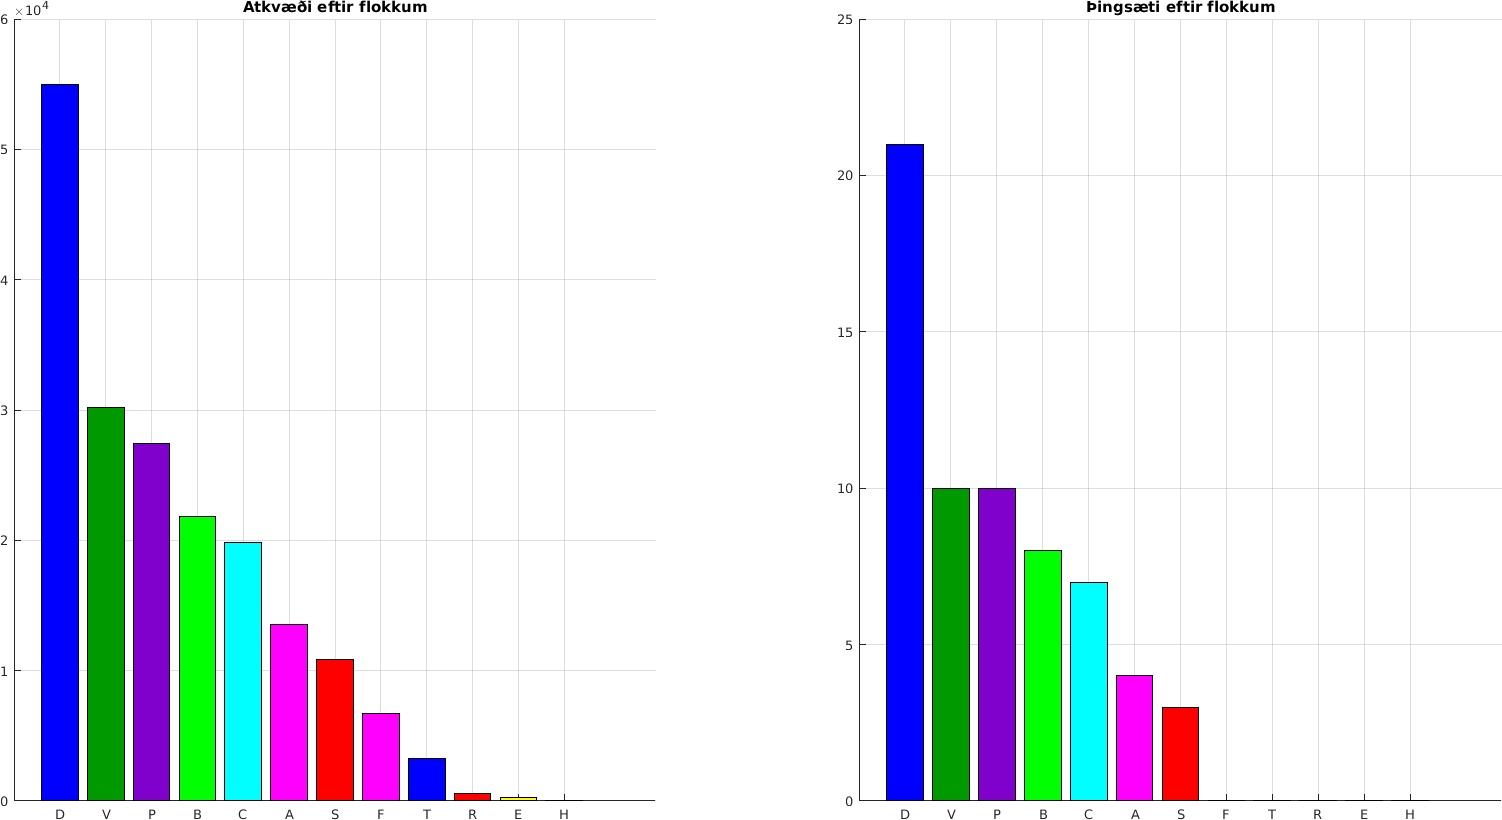
\includegraphics[width=\textwidth]{kosningar2016}
\end{frame}

\begin{frame}{Kröfur reikniritsins}
    \begin{itemize}
        \item Getum lýst inntaki og útttaki reiknirits sem úthluta á þingsætunum
        \begin{itemize}
            \item Inntak:
            \begin{itemize}
                \item Fjöldi þingsæta í kjördæmi $k$
                \item Runa atkvæðafjölda fyrir $n$ flokka, $v_1,v_2,\ldots,v_n$
            \end{itemize}
            \item Úttak:
            \begin{itemize}
                \item Runa þingsætafjölda fyrir $n$ flokka, $s_1, s_2, \ldots, s_n$
            \end{itemize}
        \end{itemize}
        \item Ætlumst til þess að þingsætafjöldinn sé ``sanngjarn''
    \end{itemize}
\end{frame}

\begin{frame}[fragile]{Möguleg útfærsla}
\begin{verbatim}
reiknirit dhondt(heiltala k, n staka heiltalnaruna v):
  // k er þingsætafjöldinn, v inniheldur atkvæðafjölda
  t = tómt n x k fylki heiltalna
  fyrir hvern flokk i:
    fyrir j frá 1 til k:
      t_ij = v_i/(j)
  s := tóm n staka runa heiltalna
  meðan summa staka s er < k:
    m = línunúmer stærsta staks í t
    s_m = s_m + 1
    yfirskrifa stærsta stakið í t með -óendanlegu
  skila s // s táknar þingsætaúthlutunina
\end{verbatim}
\end{frame}

\begin{frame}{D'Hondt tafla}
    Möguleg atkvæðadreifing í $\approx 1000$ kjósenda kjördæmi með 9 sæti.
    \begin{center}
        \begin{tabular}{cllllllllll}
            \toprule
            Flokkur&1&2&3&4&5&6&7&8&9&Sæti\\
            \midrule
            D&244& 122& 81& 61& 48& 40& 34& 30& 27&\\
            V&201& 100& 67& 50& 40& 33& 28& 25& 22&\\
            P&190&  95& 63& 47& 38& 31& 27& 23& 21&\\
            C&116&  58& 38& 29& 23& 19& 16& 14& 12&\\
            A& 76&  38& 25& 19& 15& 12& 10&  9&  8&\\
            B& 57&  28& 19& 14& 11&  9&  8&  7&  6&\\
            S& 52&  26& 17& 13& 10&  8&  7&  6&  5&\\
            F& 38&  19& 12&  9&  7&  6&  5&  4&  4&\\            
            \bottomrule
        \end{tabular}
    \end{center}
\end{frame}

\begin{frame}{D'Hondt tafla}
    Veljum 9 hæstu tölurnar til að fá þingsætadreifingu.
    \begin{center}
        \begin{tabular}{clllllllllc}
            \toprule
            Flokkur&1&2&3&4&5&6&7&8&9&Sæti\\
            \midrule
            D&\textbf{$244^1$}& \textbf{$122^4$}& \textbf{$81^8$}& 61& 48& 40& 34& 30& 27&3\\
            V&\textbf{$201^2$}& \textbf{$100^6$}& 67& 50& 40& 33& 28& 25& 22&2\\
            P&\textbf{$190^3$}& \textbf{$95^7$}& 63& 47& 38& 31& 27& 23& 21&2\\
            C&\textbf{$116^5$}&  58& 38& 29& 23& 19& 16& 14& 12&1\\
            A&\textbf{$76^9$}&  38& 25& 19& 15& 12& 10&  9&  8&1\\
            B& 57&  28& 19& 14& 11&  9&  8&  7&  6&0\\
            S& 52&  26& 17& 13& 10&  8&  7&  6&  5&0\\
            F& 38&  19& 12&  9&  7&  6&  5&  4&  4&0\\
                        
            \bottomrule
        \end{tabular}
    \end{center}
\end{frame}

\begin{frame}{Jöfnunarþingsæti}
    \begin{itemize}
        \item Auk kjördæmasæta eru jöfnunarþingsæti á Íslandi
        \begin{itemize}
            \item Tvö í Reykjavíkurkjördæmum og Suðvestur, eitt í Norðurkjördæmum og Suðurkjördæmi, samtals 9
        \end{itemize}
        \item Eingöngu flokkar sem fá 5\% atkvæða geta fengið jöfnunarþingsæti
        \begin{itemize}
            \item ``5\% múrinn'' á ekki við um kjördæmasæti
        \end{itemize}
        \item Útdeiling jöfnunarsætanna fer fram í þremur skrefum
        \begin{enumerate}
            \item Samsetning landstölulista
            \item Finna fólkið sem var næst því að komast inn í hverju kjördæmi, sett á úthlutunarskrá
            \item Útdeiling sæta
        \end{enumerate}
    \end{itemize}
\end{frame}

\begin{frame}{Samsetning landstölulista}
    \begin{columns}
        \column{0.6\textwidth}
        \begin{itemize}
            \item Notum aftur endurtekna deilingu til að setja saman landslista
            \item Fyrir hvern flokk, reikna landstölur
            \begin{itemize}
                \item Landstölur eru kvótarnir $\frac{v}{s+1}, \frac{v}{s+2},\ldots$ þar sem $v$ er fjöldi atkvæða sem flokkurinn fékk á landsvísu og $s$ er heildarfjöldi kjördæmakjörinna
            \end{itemize}
            \item Landstölulistar flokkanna eru sameinaðar í einn landstölulista
        \end{itemize}
        \column{0.4\textwidth}
        Landstölur 2016, efstu 9 sætin:
        \begin{enumerate}            
            \item S: 5446
            \item A: 4526
            \item C: 3974
            \item S: 3631
            \item A: 3394
            \item C: 3311
            \item V: 3016
            \item C: 2838
            \item P: 2744
        \end{enumerate}
    \end{columns}
\end{frame}

\begin{frame}{Úthlutunarskrá}
    \begin{columns}
        \column{0.5\textwidth}
        \begin{itemize}
            \item Í hverju kjördæmi eru næstu tveir kandídatar fundnir
            \item Reiknuð atkvæðahlutföll fyrir hvern frambjóðanda sem ekki komst inn
            \item Þau sem hafa hæstu hlutföll eru sett efst á sameinaða úthlutunarskrá
        \end{itemize}
        \column{0.5\textwidth}
        Dæmi: Úthlutunarskrá Samfylkingarinnar 2016
        \begin{enumerate}
            \tiny
            \item Oddný G. Harðardóttir (Suður): 6,38\%
            \item Guðjón S. Brjánsson (Norðvestur): 6,29\%
            \item Össur Skarphéðinsson (Reykjavík suður): 5,58\%
            \item Sigríður Ingibjörg Ingadóttir (Reykjavík norður): 5,21\%
            \item Árni Páll Árnason (Suðvestur): 4,75\%
            \item Erla Björg Guðmundsdóttir (Norðaustur): 4,0\%
            \item Ólafur Þór Ólafsson (Suður): 3,19\%
            \item Inga B. Bjarnadóttir (Norðvestur): 3,14\%
            \item Eva H. Baldursdóttir (Reykjavík suður): 2,79\%
            \item Hildur Þórisdóttir (Norðaustur): 2,67\%
            \item Helgi Hjörvar (Reykjavík norður): 2,6\%
            \item Margrét Gauja Magnúsdóttir (Suðvestur): 2,38\%        
        \end{enumerate}
    \end{columns}
\end{frame}

\begin{frame}{Útdeiling}
    \begin{columns}
        \column{0.5\textwidth}
        \begin{itemize}
            \item Við útdeilingu jöfnunarsæta er farið niður landstölulistann
            \item Fyrir hverja landstölu, efsti frambjóðandi á hlutfallslista viðkomandi flokks fundinn sem
            \begin{enumerate}
                \item Hefur ekki fengið jöfnunarsæti nú þegar
                \item Er ekki í kjördæmi þar sem jöfnunarsætin eru búin
            \end{enumerate}
        \end{itemize}
        \column{0.5\textwidth}
        Jöfnunarþingsæti 2016
        \begin{enumerate}
            \tiny
            \item Oddný G. Harðardóttir (S, Suður)
            \item Nichole Leigh Mosty (A, Reykjavík suður)
            \item Benedikt Jóhannesson (C, Norðaustur)
            \item Guðjón S. Brjánsson (S, Norðvestur)
            \item Theodóra S. Þorsteinsdóttir (A, Suðvestur)
            \item Jón Steindór Valdimarsson (C, Suðvestur)
            \item Andrés Ingi Jónsson (V, Reykjavík norður)
            \item Pawel Bartoszek (C, Reykjavík suður)
            \item Halldóra Mogensen (P, Reykjavík norður)       
        \end{enumerate}
    \end{columns}
\end{frame}

\begin{frame}{Nokkrar athuganir}
    \begin{itemize}
        \item Kerfið byggir á einföldum atkvæðaseðlum
        \begin{itemize}
            \item Einn kjósandi hefur eitt atkvæði
        \end{itemize}
        \item Kjördæmaskiptingin hefur mikil áhrif á niðurröðun
        \item Frambjóðandi getur náð kjördæmissæti þrátt fyrir að flokkurinn sé undir 5\% á landsvísu
        \item Kerfið tryggir ekki háa atkvæðanýtingu
        \item Jöfnunarþingsætakerfið er óreiðukennt (e. \emph{chaotic}) - litlar breytingar á atkvæðatölum geta haft miklar afleiðingar á uppröðun jöfnunarþingsæta
    \end{itemize}
\end{frame}

\subsection{Önnur kosningakerfi}

\begin{frame}{Önnur kosningakerfi}
    \begin{itemize}
        \item Hægt er að mynda kosningakerfi á marga vegu
        \item Dæmi um tilbrigði við hlutfallskosningaraðferð eins og D'Hondt - nota aðra kvóta
        \begin{itemize}
            \item Aðferð Websters: Kvótarnir $\frac{v}{2s+1}$ notaðir í stað $\frac{v}{s+1}$ í D'Hondt, kemur sér betur fyrir litla flokka
        \end{itemize}
        \item Getum líka myndað alveg ný kosningakerfi
    \end{itemize}
\end{frame}

\begin{frame}{Webster tafla}
    Veljum 9 hæstu tölurnar til að fá þingsætadreifingu.
    \begin{center}
        \begin{tabular}{clllllllllc}
            \toprule
            Flokkur&1&/3&/5&/7&/9&/13&/15&/17&/19&Sæti\\
            \midrule
            D&$244^1$&    $81^5$&    48&    34&    27&    18&    16&    14&    12&2\\
            V&$201^2$&    $67^7$&    40&    28&    22&    15&    13&    11&    10&2\\
            P&$190^3$&    $63^8$&    38&    27&    21&    14&    12&    11&    10&2\\
            C&$116^4$&    38&    23&    16&    12&     8&     7&     6&     6&1\\
            A&$76^6$&    25&    15&    10&     8&     5&     5&     4&     4&1\\
            B&$57^9$&    19&    11&     8&     6&     4&     3&     3&     3&1\\
            S& 52&    17&    10&     7&     5&     4&     3&     3&     2&0\\
            F& 38&    12&     7&     5&     4&     2&     2&     2&     2&0\\
            \bottomrule
        \end{tabular}
    \end{center}
\end{frame}

\begin{frame}{STV}
    \begin{columns}
        \column{0.5\textwidth}
        \begin{itemize}
            \item Raðaðir atkvæðaseðlar fela í sér ýmsa möguleika
            \item Einn slíkur möguleiki - Single Transferable Vote (STV) kerfi
            \item Kjósendur forgangsraða frambjóðendum á kjörseðlinum
            \item Hver kjósandi hefur eitt atkvæði sem getur flust yfir til annars frambjóðandi nái sá fyrsti ekki sæti
        \end{itemize}
        \column{0.5\textwidth}
        \begin{center}
            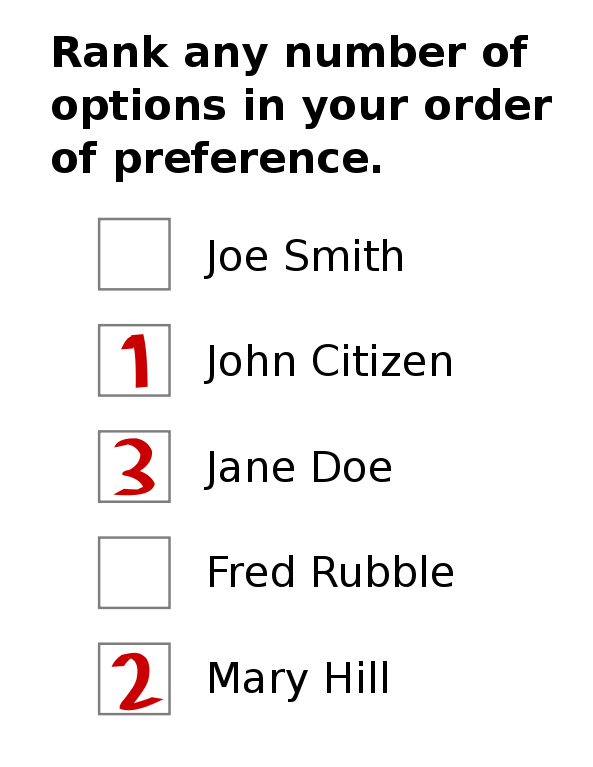
\includegraphics[width=\linewidth]{stv}
            \\
            \href{https://upload.wikimedia.org/wikipedia/commons/thumb/1/18/Preferential\_ballot.svg/593px-Preferential\_ballot.svg.png}{Kjörseðill með forgangsröðun}
        \end{center}
    \end{columns}
\end{frame}

\begin{frame}{Talning í STV}
    STV kerfi þarfnast lágmarksþröskulds til að ná kjöri, venjulega
    \[
        v_n = \left \lfloor \frac{v_t}{s+1} \right \rfloor+1
    \]
    þar sem $v_n$ er nauðsynlegur atkvæðafjöldi, $v_t$ er heildarfjöldi atkvæða sem fellur til og $s$ er sætisfjöldinn.

    \vspace{0.5cm}
    Athugum: Í einkstaklingskosningum er þetta jafngilt því að þurfa $50\%+1$ atkvæði
\end{frame}

\begin{frame}{Framkvæmd STV}
    \begin{itemize}
        \item STV kosning fer fram í nokkrum umferðum, þar sem hver umferð skiptist í skref:
        \begin{enumerate}
            \item Frambjóðandi sem nær þröskuldinum er talinn kjörinn
            \item Fái frambjóðandi fleiri atkvæði en nauðsynlegt er flytjast umframatkvæði yfir til næsta vals 
            \begin{itemize}
                \item Þetta má t.d. gera hlutfallslega eða á slembinn hátt
            \end{itemize}
            \item Hafi þessi umferð ekki bætt við neinum sem náðu kjöri er sá frambjóðandi sem hefur fæst atkvæði felldur út og atkvæði til viðkomandi færð yfir á næsta val
        \end{enumerate}
    \end{itemize}
\end{frame}

\begin{frame}{Nokkrar athuganir}
    \begin{itemize}
        \item STV getur aukið atkvæðanýtingu miðað við einfaldar hlutfallskosningar
        \item Atkvæðaseðlarnir verða flóknari
        \item Reikniritið er flóknara - minna gegnsæi
        \item Aðferðin er ekki ``monotonic''
        \begin{itemize}
            \item Það að gefa frambjóðanda lægri einkunn getur kostað viðkomandi kosningu
        \end{itemize}
    \end{itemize}
\end{frame}

\begin{frame}{Villa í STV}
    Þrír frambjóðendur (vinstri, hægri, miðja) etja kappi um eitt sæti. 100 kjósendur mæta á kjörstað og velja sína tvo uppáhalds.
    \vspace{0.5cm}
    \begin{columns}
        \column{0.5\textwidth}
        \begin{center}
            \begin{tabular}{llc}
                \toprule
                Fyrsta val&Annað val&Fjöldi\\
                \midrule
                Hægri 	&Miðja& 	28\\
                Hægri 	&Vinstri &	5\\
                Vinstri 	&Miðja& 	30\\
                Vinstri 	&Hægri &	5\\
                Miðja 	&Vinstri &	16\\
                Miðja 	&Hægri &	16\\
                \bottomrule
            \end{tabular}
        \end{center}
        \column{0.5\textwidth}
        Í einfaldri hlutfallskosningu vinnur vinstri með 35 atkvæðum. Í STV vinnur vinstri með 30+5+16=51 atkvæði gegn hægri.
    \end{columns}
\end{frame}

\begin{frame}{Villa í STV}
    Svipuð kosning, en tveir kjósendur hægri sem áður völdu vinstri sem 2. val hafa víxlað röð atkvæða og vilja þar með frekar vinstri.
    \vspace{0.5cm}
    \begin{columns}
        \column{0.5\textwidth}
        \begin{center}
            \begin{tabular}{llc}
                \toprule
                Fyrsta val&Annað val&Fjöldi\\
                \midrule
                Hægri 	&Miðja& 	28\\
                \textbf{Hægri} 	&\textbf{Vinstri} &	\textbf{3}\\
                Vinstri 	&Miðja& 	30\\
                \textbf{Vinstri} 	&\textbf{Hægri} &	\textbf{7}\\
                Miðja 	&Vinstri &	16\\
                Miðja 	&Hægri &	16\\
                \bottomrule
            \end{tabular}
        \end{center}
        \column{0.5\textwidth}
        Nú fara vinstri (37 atkvæði) og miðja (32 atkvæði) í 2. umferð. En nú sigrar miðja með 16+16+28 = 60 atkvæðum gegn 30+7+3 atkvæðum.
    \end{columns}
\end{frame}

\section{Sérstök net}

\begin{frame}{Sérstök net}
\begin{itemize}
 \item Ýmis net hafa sérstakar uppbyggingar
 \item Nefnum sérstaklega:
 \begin{itemize}
  \item Tóm net (e. \emph{empty graph})
  \item Núllnet (e. \emph{null graph})
  \item Fullskipuð net (e. \emph{complete graph})
  \item Hringa (e. \emph{cycles})
  \item Hjól (e. \emph{wheels})
  \item $n$-teningar (e. \emph{$n$-cubes})
 \end{itemize}
\end{itemize}
\end{frame}

\begin{frame}{Tóm net og núllnet}
\begin{tcolorbox}[title=Tómt net]
Tómt net er net $G = (V, E)$ þar sem $E = V = \emptyset$. Þ.e.a.s. net er tómt ef það inniheldur enga leggi og enga hnúta.
\end{tcolorbox}

\begin{tcolorbox}[title=Núllnet]
Núllnet er net $G = (V, E)$ þar sem $E = \emptyset$. Þ.e.a.s. net er núllnet ef það inniheldur enga leggi til að tengja hnúta þess saman.
\end{tcolorbox}
Ath: Nöfnunum á þessum skilgreiningum er stundum víxlað!
\end{frame}

\begin{frame}{Fullskipuð net}
\begin{tcolorbox}[title=Fullskipað net]
Fullskipað net með $n$ hnútum er einfalt net sem hefur nákvæmlega einn legg á milli hverra tveggja aðskildra hnúta. Fullskipað net með $n$ hnútum er táknað með $K_n$.
\end{tcolorbox}

\begin{center}
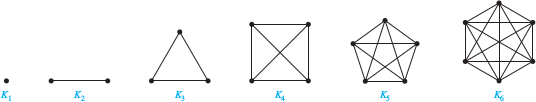
\includegraphics[width=\linewidth]{graph-complete}
\end{center}

\end{frame}

\begin{frame}{Hringur}
\begin{tcolorbox}[title=Hringur]
Hringur með $n \geq 3$ hnútum er einfalt net með hnúta $v_1, v_2, \ldots, v_n$ og leggi $\{v_1 , v_2\},
\{v_2 , v_3 \}, \ldots , \{v_{n-1} , v_n \}$, og $\{v_n , v_1 \}$. Hringur með $n$ hnútum er táknaður með $C_n$.
\end{tcolorbox}

\begin{center}
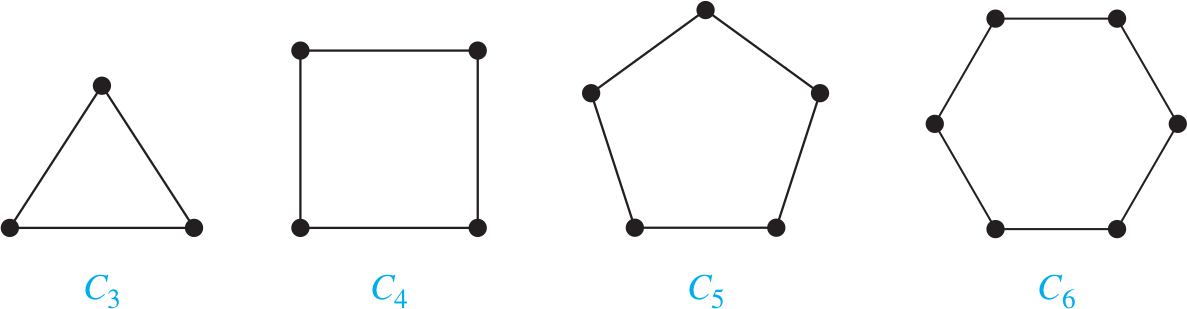
\includegraphics[width=\linewidth]{graph-cycle}
\end{center}

\end{frame}

\begin{frame}{Hjól}
\begin{tcolorbox}[title=Hjól]
Hjólið $W_n$ er myndað með því að taka hringinn $C_n$ og bæta við það einum hnúti og leggjum sem tengja nýja hnútinn við sérhvern hnút í $C_n$. Hjólið $W_n$ er þá með $n+1$ hnút.
\end{tcolorbox}

\begin{center}
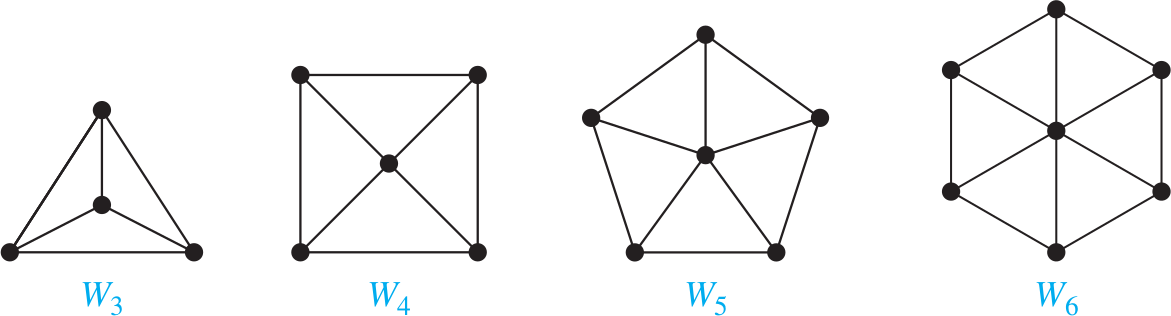
\includegraphics[width=\linewidth]{graph-wheel}
\end{center}
\end{frame}

\begin{frame}{$n$-teningur}
\begin{tcolorbox}[title=$n$-teningur]
$n$-tengingur, eða ``$n$-víður ofurteningur'' er táknaður með $Q_n$.

Látum $Q_0$ vera netið sem samanstendur af einum hnút og engum leggjum. Þá má búa til $Q_{n+1}$ út frá $Q_n$ með því að taka alla hnúta í $Q_n$, afrita þá, og bæta legg við á milli hvers upphaflegs hnúts og afrits hans.
\end{tcolorbox}

\begin{center}
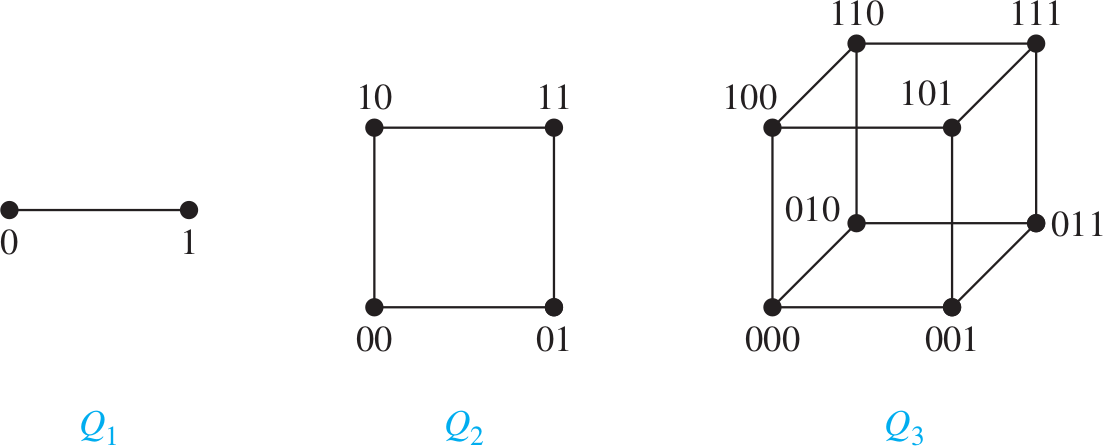
\includegraphics[width=\linewidth]{graph-n-cube}
\end{center}
\end{frame}

\section{Tvíhlutanet}

\begin{frame}{Tvíhlutanet}
Net sem kallast tvíhlutanet hafa eiginleika sem vert er að skoða sérstaklega.
\begin{tcolorbox}[title=Tvíhlutanet]
Einfalt net $G = (V,E)$ kallast tvíhlutanet (e. \emph{bipartite graph}) megi skipta $V$ í tvö aðskilin mengi $V_1$ og $V_2$ þannig að allir leggir í netinu hafa annan endapunkt sinn í $V_1$ og hinn í $V_2$. Þá mynda mengin $V_1$ og $V_2$ tvískiptingu (e. \emph{bipartition}) á hnútamengi $G$.
\end{tcolorbox}

\end{frame}

\begin{frame}{Dæmi}
Er hringurinn $C_6$ tvíhlutanet? \pause

\begin{center}
Já!

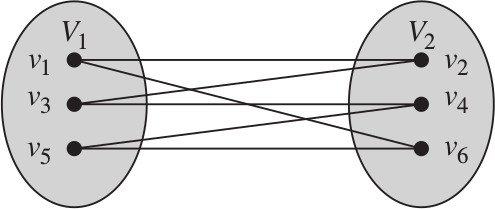
\includegraphics[width=0.8\textwidth]{graph-bipartite-c6}
\end{center}
\end{frame}

\begin{frame}{Litun á tvíhlutaneti}
Við getum inleitt hugmyndina um litun á neti (e. \emph{graph coloring}) til að auðvelda okkur að kanna hvort að net sé tvíhlutanet eða ekki.

\begin{tcolorbox}[title=Litun tvíhlutanets]
Einfalt net er tvíhlutanet þá og því aðeins að hægt sé að lita hvern hnút netsins með einum af tveimur litum á þann hátt að enginn hnútur fái sama lit og nágranni sinn.
\end{tcolorbox}

\end{frame}

\begin{frame}{Dæmi}
Eru netin $G$ og $H$ tvíhlutanet?

\begin{center}
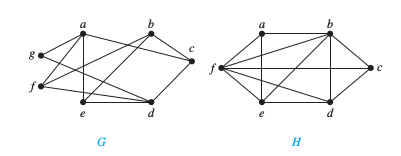
\includegraphics[width=0.8\textwidth]{graph-bipartite-coloring}
\end{center}
\pause

$G$ er tvíhlutanet, $H$ ekki.
\end{frame}

\begin{frame}{Fullskipuð tvíhlutanet}
Fullskipað tvíhlutanet $K_{m, n}$ er net sem mynda má á tvíhlutaskiptingu $\{V_1, V_2\}$ þar sem $|V_1| =m, |V_2|=n$ og með legg á milli tveggja hnúta þá og því aðeins að annar endahnútur leggsins sé í $V_1$ og hinn í $V_2$.
\end{frame}

\section{Spyrðingar}

\begin{frame}{Spyrðingar}
\begin{tcolorbox}[title=Spyrðing]
Spyrðing (e. \emph{matching}) í einföldu neti $G = (V, E)$ er hlutmengi $E$ sem hefur þann eiginleika að engir tveir leggir eigi sameiginlegan endahnút.
\end{tcolorbox}
Önnur leið til að sjá fyrir sér spyrðingu: Séu leggirnir $\{s, t\}$ og $\{u, v\}$ aðskildir leggir í spyrðingu, þá eru hnútarnir $s, t, u$ og $v$ aðskildir hnútar.
\end{frame}

\begin{frame}{Dæmi}
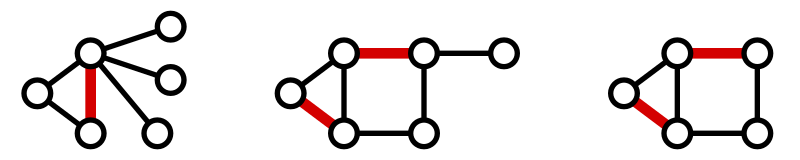
\includegraphics[width=\textwidth]{matching-maximal}
\end{frame}

\begin{frame}{Eiginleikar spyrðinga}
\begin{itemize}
 \item Spyrðing í neti er af hámarksstærð (e. \emph{maximum matching}) ef ekki er til spyrðing sem tekur til fleiri leggja í netinu
 \item Spyrðing í neti er fullkomin (e. \emph{complete}) ef sérhver hnútur í netinu er endi einhvers leggs hennar
 \begin{itemize}
  \item Bókin skilgreinir sérstaklega ákveðna gerð fullkominnar spyrðingar fyrir tvíhlutanet
  \item Spyrðing $M$ í tvíhlutanetinu $G=(V, E)$ með tvíhlutaskiptingu $\{V_1, V_2\}$ er fullkomin frá $V_1$ til $V_2$ sé sérhver hnútur í $V_1$ endahnútur einhvers leggs í spyrðingunni 
 \end{itemize}
\end{itemize}
\end{frame}

\begin{frame}{Dæmi}
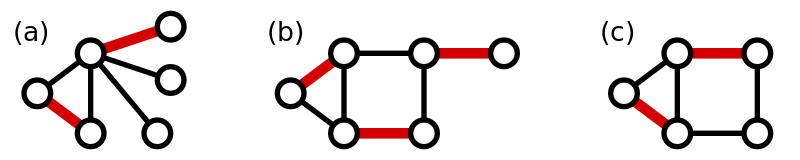
\includegraphics[width=\textwidth]{matching-maximum}
\end{frame}

\section{Framsetning á netum}

\begin{frame}{Framsetning á netum}
\begin{itemize}
 \item Það að teikna net upp er ekki alltaf vænlegur kostur
 \item Skoðum þrjá möguleika sem við höfum til að setja net fram
 \begin{itemize}
  \item Grennslalistar (e. \emph{adjacency lists})
  \item Grennslafylki (e. \emph{adjacency matrices})
  \item Legufylki (e. \emph{incidence matrices})
 \end{itemize}
\end{itemize}
\end{frame}

\begin{frame}{Grennslalistar}
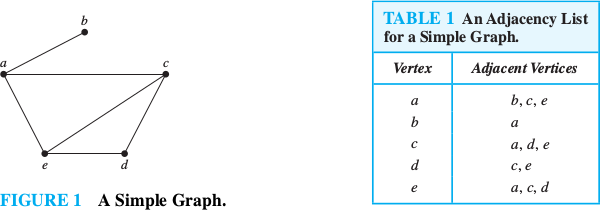
\includegraphics[width=\textwidth]{adjacency-lists}

Þessi aðferð er lítið notuð í bókinni, en er mjög venjuleg í forritun.
\end{frame}

\begin{frame}{Grennslafylki}
Látum $G = (V, E)$ vera einfalt net með $|V| = n$ og búum til röðun á hnútunum $v_1, v_2, \ldots v_n$. Legufylkið $A_G$ m.t.t. þessarar röðunar er þá $n \times n$ fylki $[a_{ij}]$ þar sem $a_{ij}$ er 1 sé $\{v_i,v_j\}$ leggur í fylkinu og 0 annars.

Dæmi, með hnútaröðunina í stafrófsröð:
\begin{center}
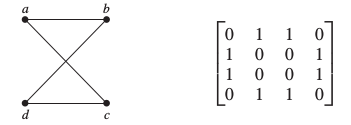
\includegraphics[width=0.6\textwidth]{adjacency-matrix}
\end{center}
Væri netið ekki einfalt gætum við sett hærri tölur í sætin. Grennslafylki fyrir stefnt net væri ekki endilega samhverft.
\end{frame}

\begin{frame}{Legufylki}
Látum $G = (V, E)$ vera óstefnt net með $V = \{v_1, v_2, \ldots, v_n\}$ og $E = \{e_1, e_2, \ldots, e_m\}$. Legufylki netsins m.t.t. þessara raðana er þá $n \times m$ fylki $[m_{ij}]$ þar sem $m_{ij}$ er 1 sé leggurinn $e_j$ tengdur hnútnum $v_i$, annars 0.

Dæmi:
\begin{center}
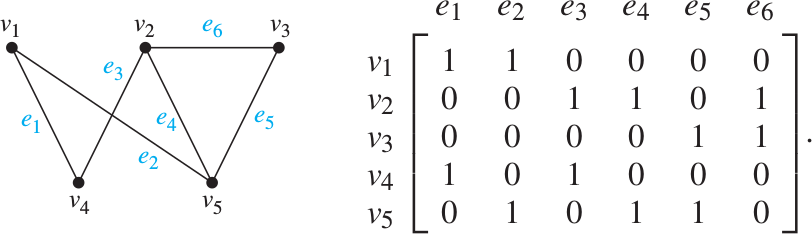
\includegraphics[width=0.6\textwidth]{incidence-matrix}
\end{center}
Lykkja myndar dálk með einum ás. Í fjölneti eru endurteknir dálkar.
\end{frame}

\begin{frame}{Næst}
Samhengi neta (10.3), kannski Euler- og Hamilton vegir (10.4).
\end{frame}


\end{document}
